%%%%%%%%%%%%%%%%%%%%%%% file typeinst.tex %%%%%%%%%%%%%%%%%%%%%%%%%%%%%%
%
% This is the LaTeX source for the instructions to authors using
% the LaTeX document class SVMultln with class option 'lnicst'
% for contributions to the Lecture Notes of the Institute for
% Computer Sciences, Social-Informatics and
% Telecommunications Engineering series.
% www.springer.com/series/XXXX       Springer Heidelberg 2007/08/05
%
% It may be used as a template for your own input - copy it
% to a new file with a new name and use it as the basis for
% your article. It contains a few tweaked sections to demonstrate
% features of the package, though.
%
% If you have not much experiences with Springer LaTeX support,
% you should better use the special demonstration file "lnicst.tex"
% included in the LaTeX package for LNICST as template.
%
%%%%%%%%%%%%%%%%%%%%%%%%%%%%%%%%%%%%%%%%%%%%%%%%%%%%%%%%%%%%%%%%%%%%%%%%

%\documentclass[lnicst,sechang,a4paper]{svmultln}
\documentclass{llncs} %this is for NSS
\bibliographystyle{splncs3}
%\documentclass[runningheads,a4paper]{llncs} 



\usepackage{amssymb}
\setcounter{tocdepth}{3}
\usepackage{graphicx}


%\usepackage{amssymb}
%\setcounter{tocdepth}{3}
%\usepackage{graphicx}
%\usepackage{fancyhdr}
%\usepackage{lastpage}

\usepackage{url}

%\urldef{\mailsa}\path|{alfred.hofmann, ursula.barth, ingrid.haas, frank.holzwarth,|
%\urldef{\mailsb}\path|anna.kramer, leonie.kunz, christine.reiss, nicole.sator,|
%\urldef{\mailsc}\path|erika.siebert-cole, peter.strasser, lncs}@springer.com|    
%\newcommand{\keywords}[1]{\par\addvspace\baselineskip
%\noindent\keywordname\enspace\ignorespaces#1}


%added by the author himself
\usepackage{subfig}

\usepackage{color}
%\usepackage[numbers]{natbib}
\usepackage{calc}
\usepackage{siunitx}
\DeclareSIUnit\mt{\milli\tesla} %% A method for say short cut or new unit!
\sisetup{inter-unit-product = {-}}

\newcolumntype{P}[1]{>{\centering\arraybackslash}p{#1}}

\usepackage[T1]{fontenc}
\usepackage[ansinew]{inputenc}
\usepackage[english]{babel}
\usepackage{adjustbox}
\usepackage{amsmath,amsfonts,amssymb}
\usepackage{xparse}
\usepackage[section]{placeins} 
\usepackage[misc]{ifsym}
\usepackage{url}

 
\usepackage[many]{tcolorbox}
\usetikzlibrary{decorations.pathreplacing}

%added by kimmo
%\setlength\parskip{12pt}
%\setlength\parindent{0pt}
%\pagestyle{fancy}
%\fancyhf{} 
%\fancyfoot[C]{\thepage\ / \pageref{LastPage}}
%\renewcommand{\headrulewidth}{0pt}



\begin{document}



\mainmatter  % start of an individual contribution

% first the title is needed
\title{Defeating IMSI-Catchers Using Pseudonyms: A DDoS Attack and Solution}
%Concealing IMSI in 5G Network Using Identity Based Cryptography

% a short form should be given in case it is too long for the running head
%\titlerunning{Concealing IMSI Using Identity Based Encryption} 


% the name(s) of the author(s) follow(s) next
%
% NB: Chinese authors should write their first names(s) in front of
% their surnames. This ensures that the names appear correctly inlso
% the running heads and the author index.
%
\author{Mohsin Khan$^\text{1(\Letter)}$%
%%\thanks{Please note that the LNICST Editorial assumes that all authors have used
%%the western naming convention, with given names preceding surnames. This determines
%%the structure of the names in the running heads and the author index.}%
\and Kimmo J\"arvinen$^\text{1}$
\and Philip Ginzboorg$^\text{2}$
\and Valtteri Niemi$^\text{1}$
}  %

%\authorrunning{Mohsin Khan \and Valtteri Niemi}

% (feature abused for this document to repeat the title also on left hand pages)

% the affiliations are given next
\institute{$^\text{1}$University of Helsinki, Helsinki, Finland\\
\{\email{mohsin.khan, kimmo.u.jarvinen, valtteri.niemi}\}\email{@helsinki.fi}\\
$^\text{2}$ Huawei Technolgies\\
\email{philip.ginzboorg@huawei.com}
%P.O. Box 68 (Gustaf H\"allstr\"omin katu 2b)\\
%FI-00014 University of Helsinki\\
%Finland\\
%\url{https://www.cs.helsinki.fi/en}
}

%relationship stu
%
% NB: a more complex sample for affiliations and the mapping to the
% corresponding authors can be found in the file "lnicst.dem",
% that is contained in the LNICST LaTeX support package.
%

%%%\toctitle{Lecture Notes in Computer Science}
%%%\tocauthor{Authors' Instructions}
\maketitle


\begin{abstract}
Pseudonym based solutions to defeat IMSI-catchers have been published in the recent years. No fatal vulnerability in these solutions has been reported until this month. However, we have found one vulnerability. The vulnerability enables an attacker to convince the home network (HN) to forget an old pseudonym of a legitimate UE and compute a new one. The attacker does not need any participation of the legitimate UE to mount this attack. A malicious UE or a serving network (SN) can exploit this vulnerability to kick a legitimate UE out of service. We show that, exploiting this vulnerability, a novel DDoS attack can be mounted against an entire cellular network. The attack can send 50 percent of the UEs out of service using a reasonably large botnet of mobile users. We justify our claim by an analytical argument backed by a simulation. Even though, in principle, a malicious SN can also exploit the vulnerability, we argue that the SN can not gain anything meaningful before the attack is detected and stopped. Besides, an SN can behave maliciously in other even more fatal ways. Hence it is not important to protect against a malicious serving network in this context. We present a solution to fight against the DDoS attack by piggybacking the location update message sent by the serving network to the home network. We present a qualitative analysis of our solution. We argue that our solution is immune to the the DDoS attack and still protects the identity privacy, and remains backward compatible with the legacy networks. We also discuss other practical issues of the usability of pseudonyms from charging and lawful interception point of view that appear to be ignored so far.
\keywords{3GPP $\cdot$ IMSI-catchers $\cdot$ Pseudonym $\cdot$ Idenity $\cdot$ Privacy}
\end{abstract}


\section{Introduction} \label{intro}
International mobile subscriber identity (IMSI) is the global identifier of a mobile phone subscriber. IMSI-catchers are devices that can create a list of IMSIs of the subscribers present in a certain geographical area. IMSI catching is an identity privacy problem. The problem has been known for long but still prevailing in all the 3GPP defined cellular networks (GSM, UMTS, LTE) for decades \textcolor{red}{cite}. 

\subsubsection{How IMSI-catchers catch IMSI?} A subscriber's user equipment (UE) has to identify itself to the network before connecting. The identification message has to be sent in plain-text because the security of the network is based on symmetric key cryptography \textcolor{red}{cite}. In symmetric key cryptography, a secret key has to be shared before starting any encryption. The home network (HN) stores a secret key for every subscriber in the subscriber database. The secret keys are also securely stored in the respective subscriber identity module (SIM). However, the HN needs to know the identity of the subscriber to choose the right secret key to start encrypting or decrypting any message. So, when an unknown UE appears, the network makes an IMSI inquiry to the UE . Consequently, the UE has to sent the IMSI in plain-text \textcolor{red}{cite}. 

A passive IMSI-catcher who is just listening to the radio channel can read the identification message. An active IMSI-catcher who sets up a fake base station and impersonates a legitimate serving network (SN), do an IMSI inquiry to all the UEs that try to connect. The UEs respond with their respective IMSIs in plain-text \textcolor{red}{cite}. See Figure \ref{fig:IMSI-catching}. 

\begin{figure}[!tbp]
  \centering
  \begin{minipage}[b]{0.4\textwidth}
    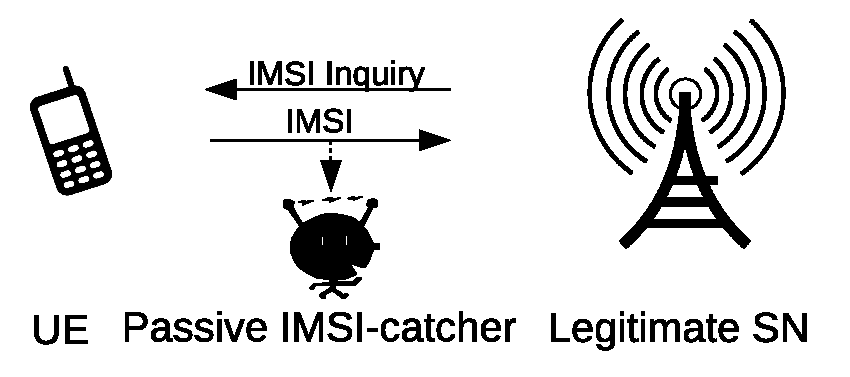
\includegraphics[width=\textwidth]{Passive_IMSI-Catcher.eps}
%    \caption{Legitimate SN}
  \end{minipage}
  \hfill
  \begin{minipage}[b]{0.57\textwidth}
    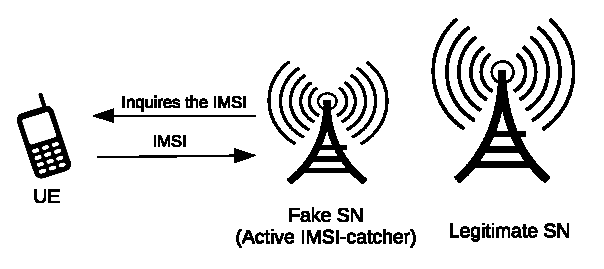
\includegraphics[width=\textwidth]{Active-IMSI-Cactcher.eps}
%    \caption{IMSI-catcher}
  \end{minipage}
  \caption{IMSI-catcher}
  \label{fig:IMSI-catching}
\end{figure}

\subsubsection{What an IMSI catcher can do with the caught IMSIs?} With the caught IMSIs, an IMSI catcher can monitor who are coming and leaving a certain geographical area \textcolor{red}{cite}. An IMSI catcher can also track the locations of a targeted individual \textcolor{red}{cite}. There are other range of more sophisticated active man in the middle attacks that start with catching the IMSI of a subscriber, e.g., attacking the confidentiality of user data by downgrading the air interface encryption \textcolor{red}{cite}. Now a days, all these advanced attackers are called IMSI-catchers. However, in this paper, we will limit our discussion to the attackers who only gathers a list of IMSIs.

\subsubsection{How available IMSI-catchers are in real life?}

\subsubsection{Current state of art in defeating IMSI-catchers}

\subsubsection{Our Contribution}

\subsubsection{Overview}



\section{Conclusion}
\label{sec:conclusion}


\subsubsection{Acknowledgement.}
\label{sec:acknowledgement}


%\bibliographystyle{splncs}
%\bibliography{mybib}{}

\begin{thebibliography}{5}



\end{thebibliography}

\end{document}
